% =============================================================================
% DATASETS SECTION
% =============================================================================

\subsection{Datasets}
\label{sec:datasets}

We evaluate our extensions on two biomedical translation quality datasets introduced by~\citet{ki-etal-2025-askqe}.

\paragraph{BioMQM (Primary).}
Our primary evaluation is conducted on BioMQM, a biomedical machine translation dataset annotated by professional translators according to the Multidimensional Quality Metrics (MQM) framework. The dataset comprises 5{,}216 sentence-level instances spanning five language pairs: English--German (en-de), English--Spanish (en-es), English--French (en-fr), English--Russian (en-ru), and English--Chinese (en-zh). Each instance includes the English source sentence, the machine-translated target, a backtranslation into English, and one or more MQM severity labels drawn from four levels: \textit{Neutral} (no error), \textit{Minor}, \textit{Major}, and \textit{Critical}. This severity stratification enables a fine-grained analysis of how each pipeline variant responds to translation errors of varying impact. Figures~\ref{fig:f1_severity},~\ref{fig:em_severity}, and~\ref{fig:sbert_severity} illustrate the baseline performance distribution across severity levels and language pairs, showing a clear degradation trend from Neutral to Critical errors across all metrics.

\paragraph{ContraTICO (Appendix).}
We additionally experiment with ContraTICO, a contrastive dataset of synthetic translation errors in the COVID-19 domain, constructed by perturbing reference translations with controlled linguistic perturbations (e.g., omission, alteration, synonym substitution). While ContraTICO provides a useful controlled setting for ablation studies, we relegate its detailed analysis to Appendix~\ref{sec:appendix_contratico} and focus the main discussion on BioMQM, which better reflects naturally occurring translation errors in a real-world biomedical setting.

\begin{figure}[htbp]
    \centering
    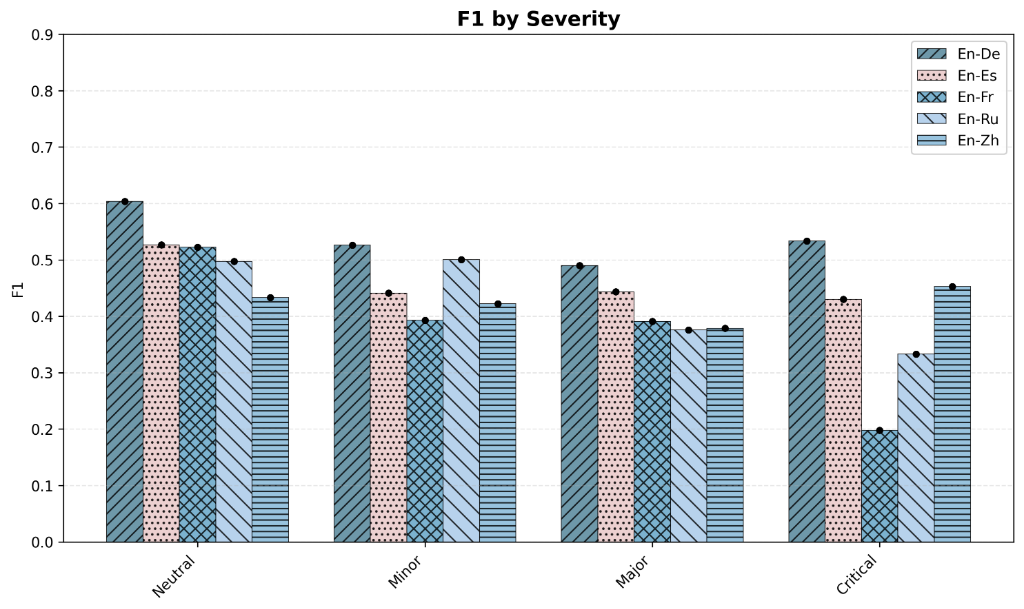
\includegraphics[width=\columnwidth]{figures/f1_by_severity.png}
    \caption{Baseline F1 scores by MQM error severity across all five language pairs. Performance decreases consistently from Neutral to Critical, with En-De exhibiting the highest scores across all severity levels.}
    \label{fig:f1_severity}
\end{figure}

\begin{figure}[htbp]
    \centering
    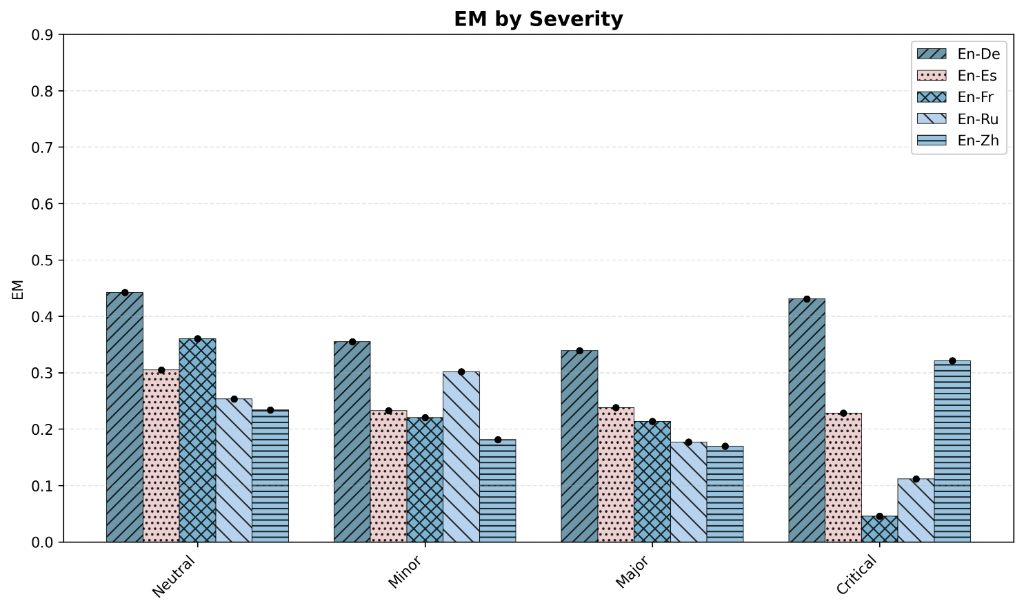
\includegraphics[width=\columnwidth]{figures/em_by_severity.png}
    \caption{Baseline Exact Match scores by severity. The trend mirrors F1, with a sharper decline for Critical errors, particularly for En-Fr and En-Ru.}
    \label{fig:em_severity}
\end{figure}

\begin{figure}[htbp]
    \centering
    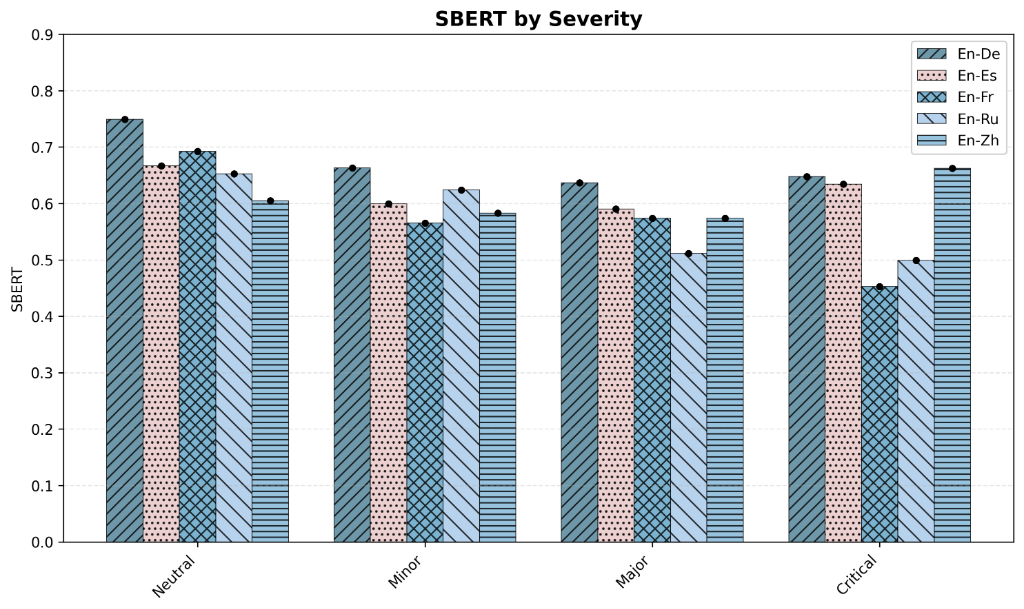
\includegraphics[width=\columnwidth]{figures/sbert_by_severity.png}
    \caption{Baseline SBERT cosine similarity by severity. Semantic similarity is more resilient than lexical metrics, yet still shows a downward trend from Neutral to Major errors.}
    \label{fig:sbert_severity}
\end{figure}
